\documentclass[10pt]{article}

\usepackage{mathtools}  % need for math tools
\usepackage{amsmath}    % need for subequations
\usepackage{graphicx}   % need for figures
\usepackage{verbatim}   % useful for program listings
\usepackage{color}      % use if color is used in text
\usepackage{subfigure}  % use for side-by-side figures
\usepackage{hyperref}   % use for hypertext links, including those to external documents and URLs


\setlength{\baselineskip}{16.0pt}   
\setlength{\parskip}{3pt plus 2pt}
\setlength{\parindent}{20pt}
\setlength{\oddsidemargin}{0.5cm}
\setlength{\evensidemargin}{0.5cm}
\setlength{\marginparsep}{0.75cm}
\setlength{\marginparwidth}{2.5cm}
\setlength{\marginparpush}{1.0cm}
\setlength{\textwidth}{150mm}

\begin{document}

\begin{center}
{\large Ay190: Computational Astrophysics (Winter Term 2012)} \\
{\large HomeWork - 7 } \\
\copyright 2012 by Arya Farahi \\
Feb 7, 2012
\end{center}

\section{Exercise 1. Solving the Poisson Equation}


\begin{figure}[hbt]
  \begin{center}
    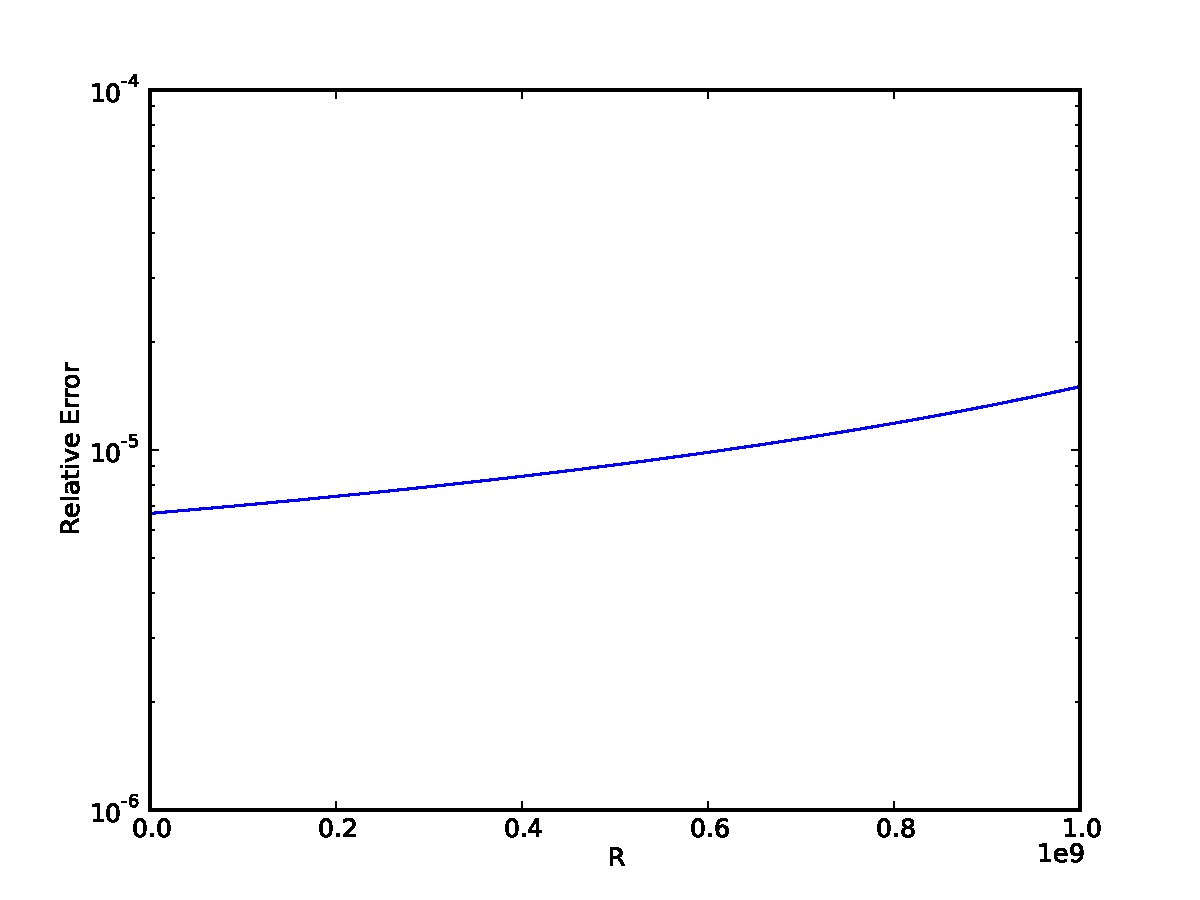
\includegraphics[scale=0.4]{Plots/Plot1.pdf}
    \caption{\label{fig:1} Plot of the relative error for grid size = 10000 point and ODE method.}
  \end{center}
\end{figure}

\begin{figure}[hbt]
  \begin{center}
    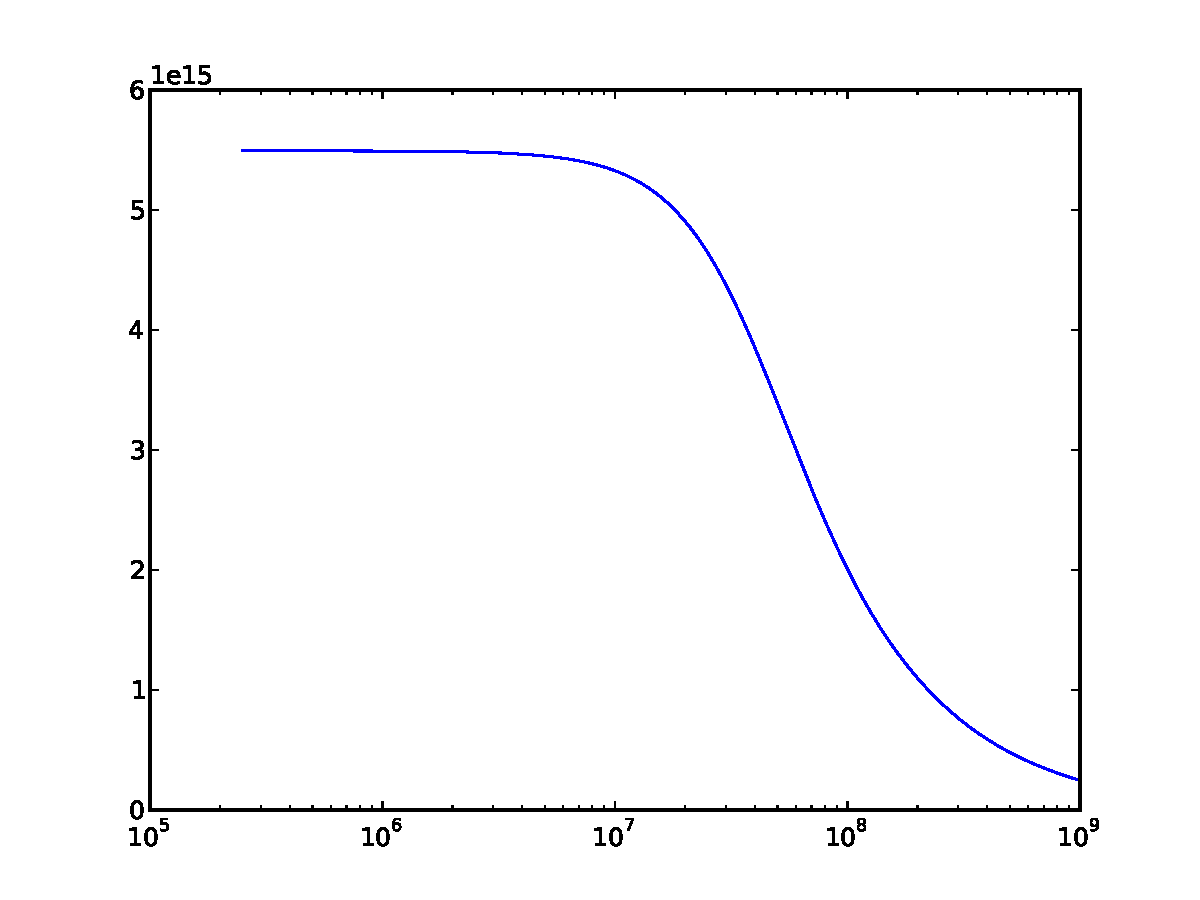
\includegraphics[scale=0.4]{Plots/plot3.pdf}
    \caption{\label{fig:2} Plot of changing of the field with radius.}
  \end{center}
\end{figure}

\begin{figure}[hbt]
  \begin{center}
    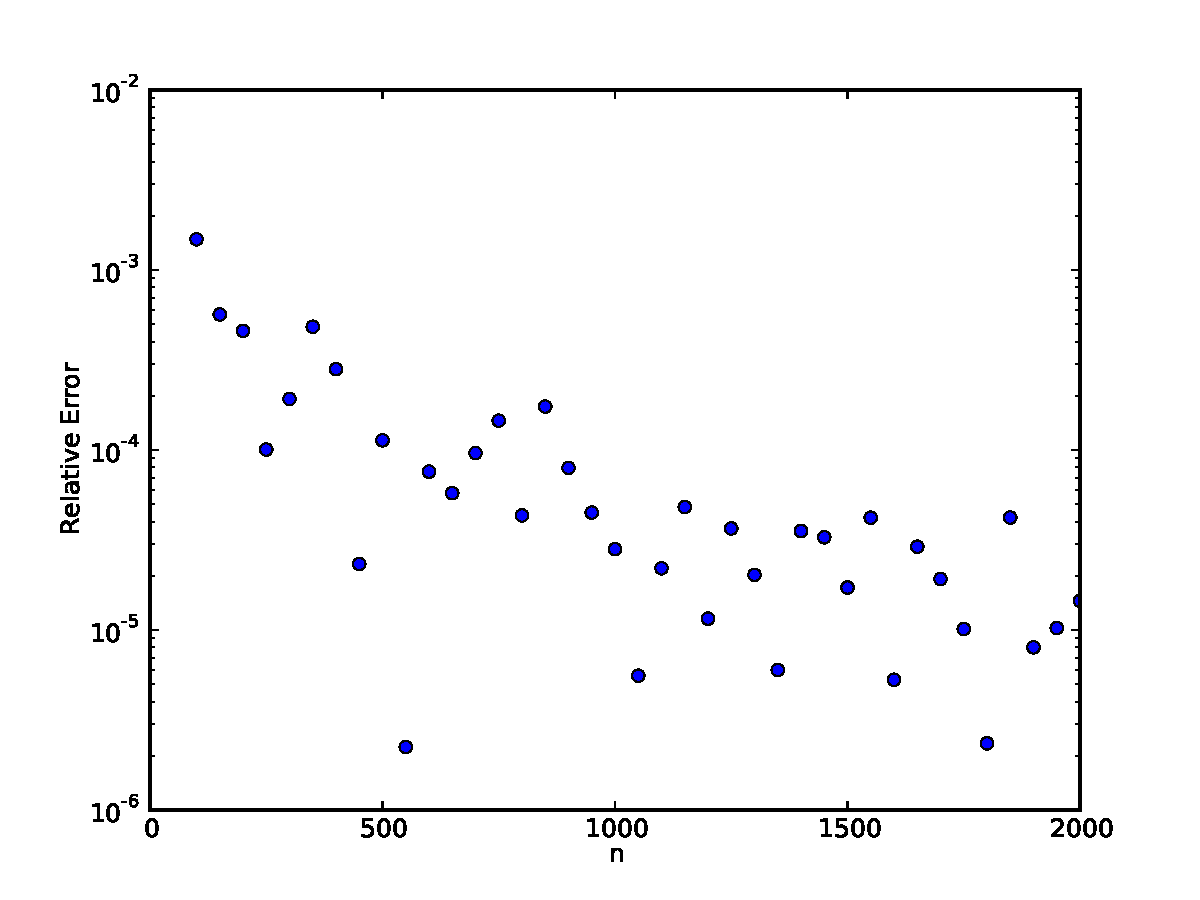
\includegraphics[scale=0.4]{Plots/plot5.pdf}
    \caption{\label{fig:3} Plot of changing of the relative error with grid size (Direct Matrix Method).}
  \end{center}
\end{figure}

Figure \ref{fig:1} and \ref{fig:3} shows the relative error of ODE method and Direct Matrix ethod in two different context. One of them is showed for one grid size which changing of radius and the other one is showed for differnet grid size but for one point. By relative error analysis it would be possible to show that for both method our solution is converging. But for direct matrix method the solution would have some flactuation but it is converging.\\

It seems that for this specific problem ODE method is much more better than the other one, because first of all it converge to real answer much more faster than the other one. Also for a large grid sizes the matrix method is too slow rather than ODE method. So it would be better to use ODE method for saving time and getting more accurate answers. \\ 

Figure \ref{fig:2} shows the changing of the field with radius for this specific problem. And the answer is the same for both method so they overlap each other. \\
\pagebreak




\end{document}
